\chapter{KẾT QUẢ THỰC NGHIỆM}

\section{Kết quả thực nghiệm trên phần cứng}
\label{sec:hw-results}

Hệ thống đo nhiệt độ và cảnh báo ngưỡng sử dụng vi điều khiển ATmega16 và cảm biến DHT11 đã được lắp ráp, nạp mã thực thi và kiểm thử thực tế trên Kit phát triển AVR tại phòng thí nghiệm Trường Điện -- Điện tử, Đại học Bách khoa Hà Nội. Các trạng thái chức năng ghi nhận trong quá trình thử nghiệm được tổng hợp dưới đây; phạm vi và giới hạn của phép kiểm chứng được trình bày ở mục \ref{sec:limitations}.

\subsection{Giai đoạn khởi động và màn hình chào mừng}
Khi vừa cấp nguồn nuôi 5V từ cổng nạp USB, vi điều khiển hoàn tất quá trình reset phần cứng, tắt cổng JTAG nội, thiết lập chiều cổng I/O và cấu hình màn hình LCD. Sau khi khởi tạo, màn hình LCD 1602 hiển thị thông điệp chào mừng khởi động:
\LCDbox{DA2: DO NHIET DO}{DHT11 SENSOR}
Màn hình duy trì thông điệp này trong khoảng 1,5 giây theo trễ phần mềm. Trong suốt giai đoạn khởi động, toàn bộ 5 đèn LED cảnh báo trên các chân PD0 -- PD4 đều tắt nhờ lệnh khởi tạo kéo mức 1 (\texttt{PORTD |= 0x1F}). Sau 1,5 giây, lệnh xóa màn hình (\texttt{0x01}) được phát ra để chuẩn bị cho chu trình hiển thị dữ liệu đo lường.

\subsection{\texorpdfstring{Trạng thái đo lường bình thường ($T < 30^\circ\text{C}$)}{Trạng thái đo lường bình thường (T < 30 °C)}}
Ở trạng thái không cảnh báo, giá trị được ghi nhận trên LCD là $26.5^\circ\text{C}$ (nhỏ hơn ngưỡng cài đặt $30^\circ\text{C}$):
\begin{itemize}[leftmargin=1.2cm]
    \item Cảm biến DHT11 thu thập dữ liệu và gửi gói tin 40-bit về MCU. Quá trình kiểm tra tính toàn vẹn dữ liệu bằng mã Checksum thành công, dữ liệu nhận được hợp lệ.
    \item \begin{samepage}Màn hình LCD 1602 hiển thị thông số:
    \LCDbox{Temp: 26.5 \textdegree C}{HIGH Th: 30\textdegree C}
    \end{samepage}
    \item Do giá trị nhiệt độ nhận được nhỏ hơn ngưỡng cài đặt, dòng 2 hiển thị ngưỡng \texttt{"HIGH Th: 30°C"} mà không xuất hiện bất kỳ dấu hiệu cảnh báo nào.
    \item Dàn 5 LED cảnh báo nối với các chân PD0 -- PD4 tiếp tục được giữ ở mức logic 1, nghĩa là tắt.
\end{itemize}

\subsection{\texorpdfstring{Trạng thái cảnh báo vượt ngưỡng quá nhiệt ($T \ge 30^\circ\text{C}$)}{Trạng thái cảnh báo vượt ngưỡng quá nhiệt (T ≥ 30 °C)}}
Để kiểm thử phản ứng của hệ thống khi có sự cố quá nhiệt, người thực hiện sử dụng nguồn nhiệt gián tiếp (hơi ấm nhẹ áp gần bề mặt cảm biến DHT11). Khi giá trị nhiệt độ nhận được đạt hoặc vượt $30.0^\circ\text{C}$:
\begin{itemize}[leftmargin=1.2cm]
    \item Vi điều khiển phát hiện điều kiện $temp\_int \ge 30^\circ\text{C}$ ở chu kỳ đọc hợp lệ tiếp theo (mỗi vòng lặp có trễ phần mềm 2 giây, cộng thời gian đọc và hiển thị).
    \item Màn hình LCD cập nhật trạng thái báo động tương ứng:
    \LCDbox{Temp: 31.5 \textdegree C}{HIGH Th: 30\textdegree C *!}
    Trên dòng 2 xuất hiện chuỗi ký hiệu báo động \texttt{"*!"} để báo cho người vận hành.
    \item Đồng thời, phép toán che mặt nạ \texttt{PORTD \&= 0xE0} kéo 5 chân PD0 -- PD4 xuống mức 0, làm 5 LED cảnh báo cùng sáng.
    \item Khi nguồn nhiệt được rút ra và giá trị nhiệt độ nhận được giảm trở lại dưới $30.0^\circ\text{C}$, màn hình tự động xóa ký hiệu \texttt{"*!"} và dàn đèn LED tự động tắt, trả hệ thống về trạng thái giám sát bình thường mà không cần thao tác reset thủ công.
\end{itemize}

\begin{figure}[H]
    \centering
    \begin{subfigure}[b]{0.46\textwidth}
        \centering
        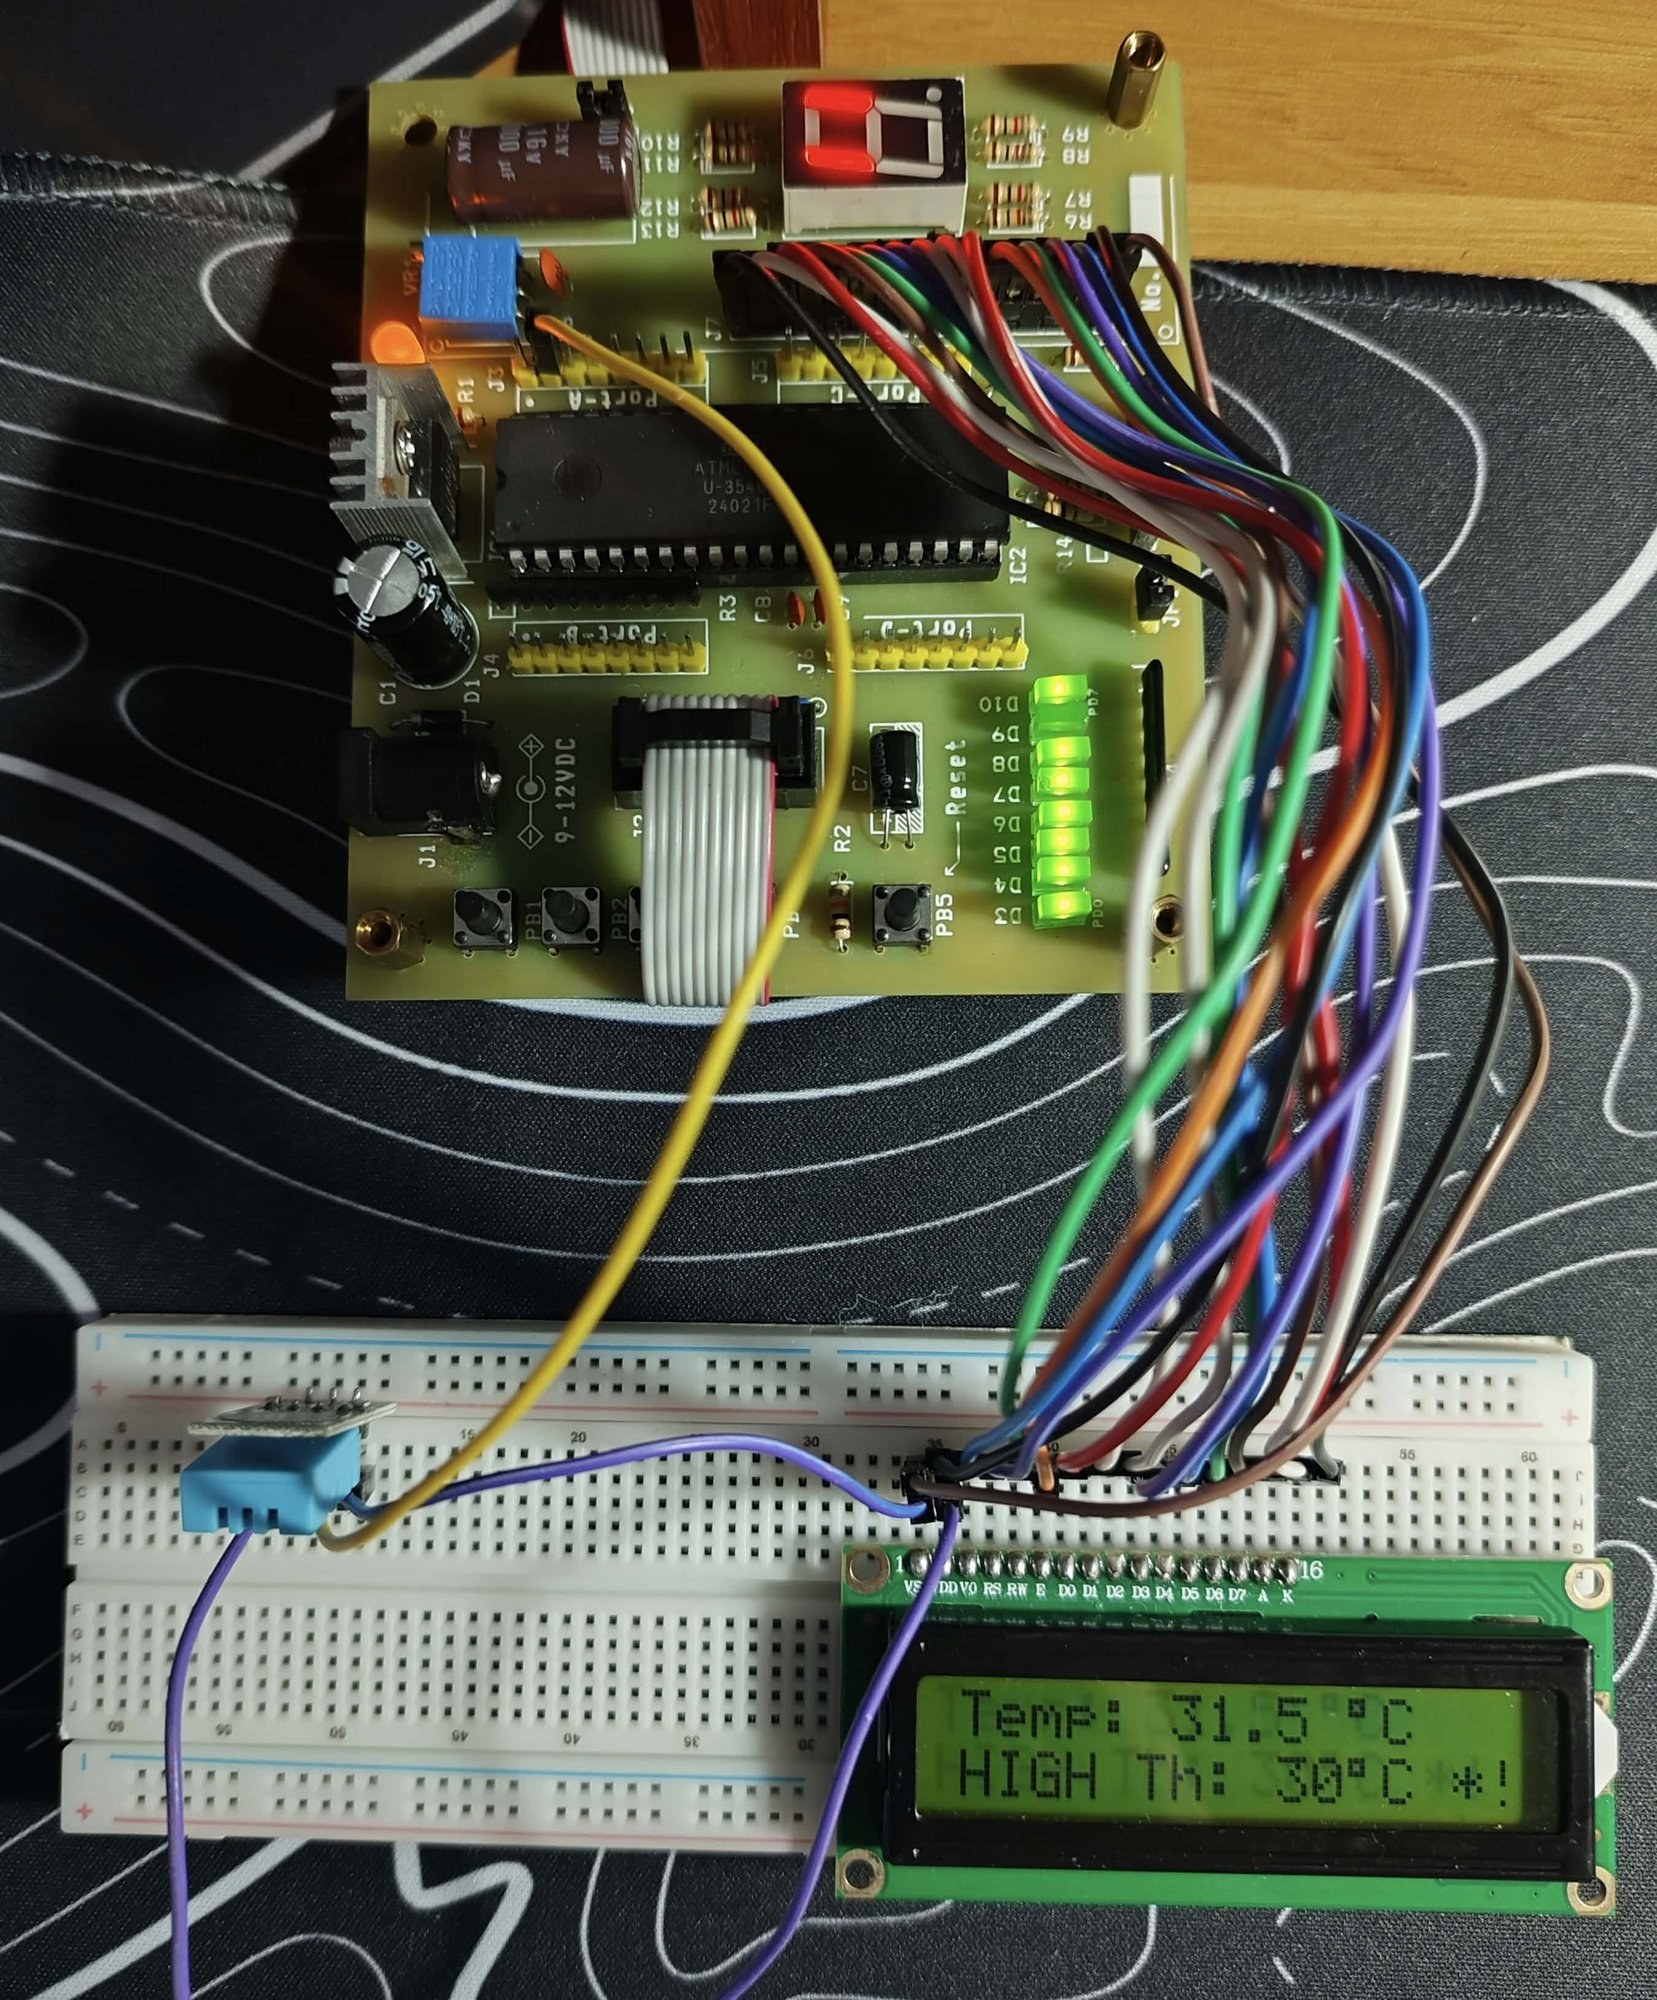
\includegraphics[height=7.5cm,keepaspectratio]{actual_system.jpg}
        \caption{Màn hình LCD khi cảnh báo quá nhiệt ($31.5^\circ\text{C}$)}
        \label{fig:actual-overheat}
    \end{subfigure}
    \hfill
    \begin{subfigure}[b]{0.46\textwidth}
        \centering
        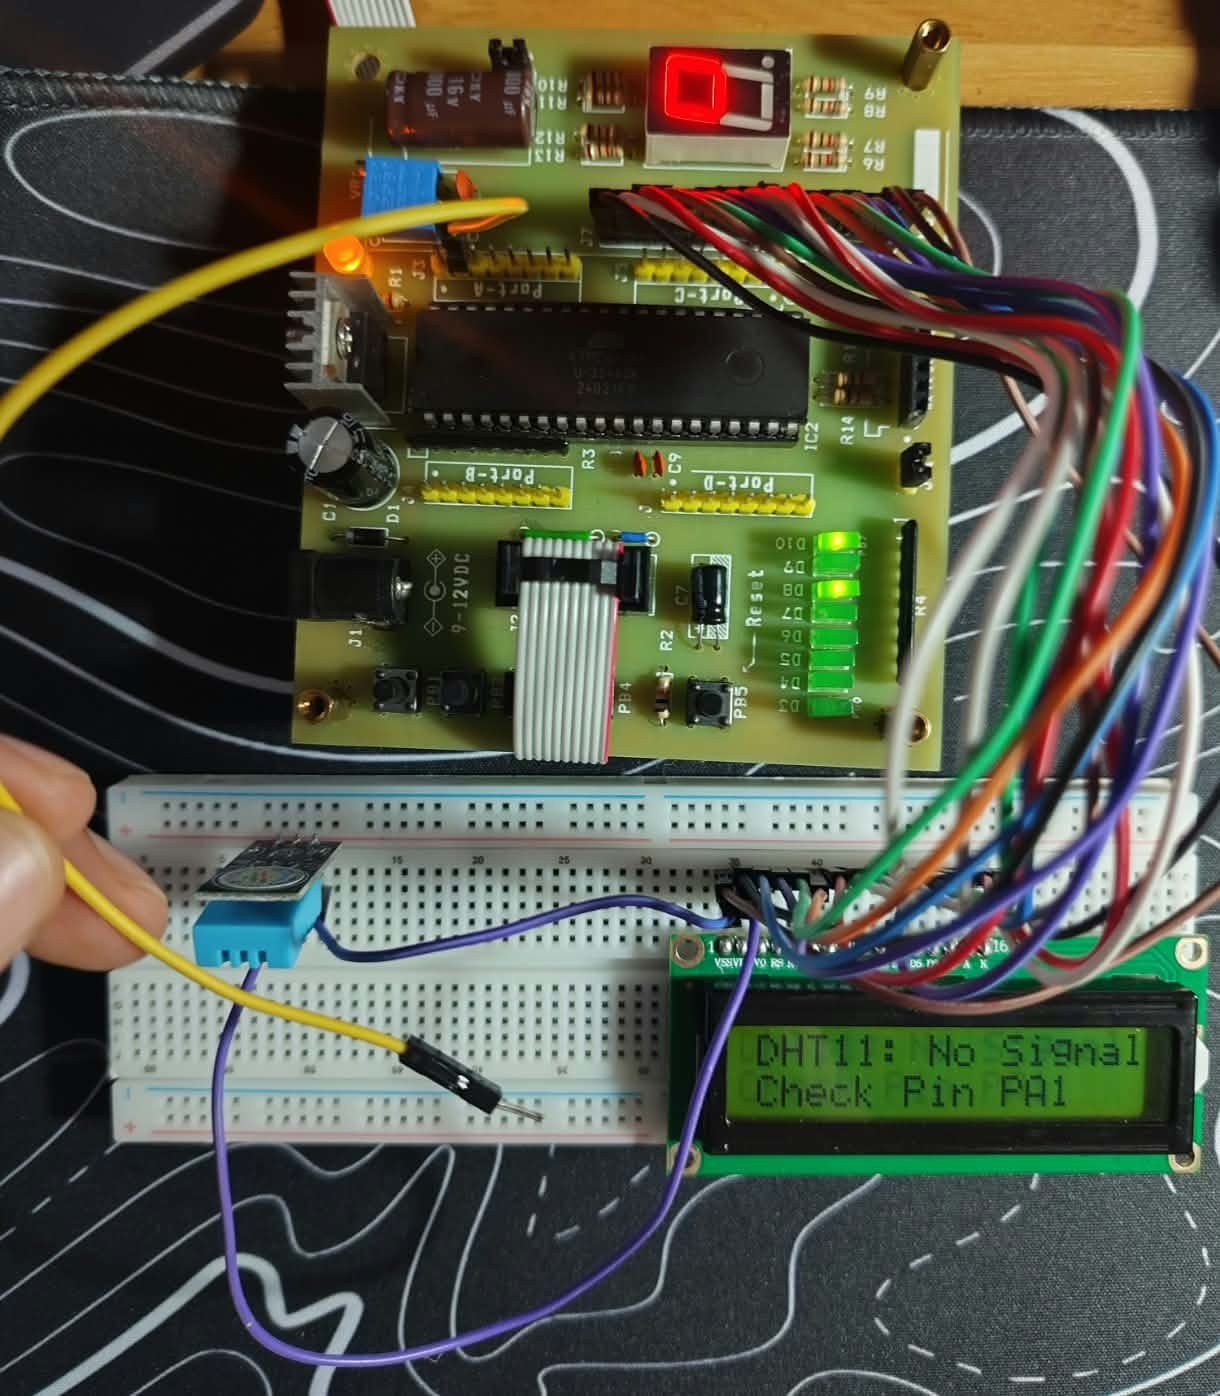
\includegraphics[height=7.5cm,keepaspectratio]{sensor_disconnect.jpg}
        \caption{Màn hình LCD khi không có tín hiệu từ cảm biến}
        \label{fig:actual-disconnect}
    \end{subfigure}
    \caption{Hình ảnh thực tế hệ thống vận hành trong các kịch bản thử nghiệm}
    \label{fig:actual-system}
    \vspace{0.1cm}
    {\small\textit{Ghi chú:} Dãy LED trên kit gồm 8 LED nối PD0--PD7 (từ D3 ở dưới lên D10 ở trên). Ba LED trên cùng (PD5--PD7) dùng chung đường RW, RS, EN của LCD nên sáng theo mức logic của các tín hiệu này, không thuộc khối cảnh báo. Ở (a), 5 LED cảnh báo PD0--PD4 sáng; ở (b), 5 LED này tắt.\par}
\end{figure}

\subsection{Kiểm tra phản hồi khi mất cảm biến và xử lý lỗi hệ thống}
Nhằm kiểm tra độ tin cậy và khả năng tự bảo vệ của hệ thống trước các tình huống bất thường, nhóm đã tiến hành xác minh theo hai cấp độ:
\begin{itemize}[leftmargin=1.2cm, topsep=0pt, itemsep=0.5pt, parsep=0pt]
    \item Thử nghiệm thực tế khi mất cảm biến (Kiểm chứng phần cứng): Để mô phỏng sự cố tuột dây tín hiệu, nhóm chủ động rút chân DATA (PA1). Vòng chờ đầu tiên của \texttt{DHT11\_Read} hết hạn và hàm trả về $-1$ sau khoảng 29\,ms (Bảng \ref{tab:timeout}); vi điều khiển không bị treo. Màn hình LCD cập nhật thông báo chẩn đoán lỗi sau khi hàm đọc cảm biến phát hiện timeout (Hình \ref{fig:actual-disconnect}):
    \LCDbox{DHT11: No Signal}{Check Pin PA1}
    \item Kiểm chứng giải thuật xử lý Checksum (Phân tích mã nguồn): Đối với trường hợp đường truyền bị can nhiễu, do chưa có thiết bị tạo xung nhiễu chuyên dụng, nhánh xử lý sai Checksum hiện chỉ được đối chiếu với luồng logic mã nguồn (nhánh \texttt{status == -6}). Thuật toán nhận diện sự sai lệch tổng kiểm tra và hiển thị thông báo chuẩn 16 ký tự:
    \LCDbox{DHT11: Sum Error}{Checksum Invalid}
    \item Trạng thái xử lý lỗi xác định: Trong cả hai tình huống, dàn 5 LED được đưa về trạng thái tắt (\texttt{PORTD |= 0x1F}) như phân tích ở mục \ref{sec:main-algo}.
\end{itemize}

\begin{table}[H]
\centering
\small
\setlength{\tabcolsep}{3pt}
\caption{Bảng tổng hợp các kịch bản kiểm tra và kết quả đánh giá hệ thống}
\label{tab:system-results}
\renewcommand{\arraystretch}{1.15}
\begin{tabularx}{\textwidth}{>{\bfseries\raggedright\arraybackslash}p{2.6cm} >{\raggedright\arraybackslash}p{2.6cm} >{\centering\arraybackslash}p{1.5cm} >{\raggedright\arraybackslash}X >{\centering\arraybackslash}p{1.8cm}}
\toprule
\textbf{Kịch bản kiểm tra} & \textbf{Phương pháp xác minh} & \textbf{Giá trị LCD} & \textbf{Nội dung hiển thị trên LCD 1602} & \textbf{Trạng thái dàn LED} \\
\midrule
Khởi động hệ thống & Thực nghiệm trên kit & -- & Dòng 1: \mbox{\texttt{DA2: DO NHIET DO}}\newline Dòng 2: \mbox{\texttt{DHT11 SENSOR}} & Tắt toàn bộ \\
\midrule
Nhiệt độ bình thường & Thực nghiệm trên kit & $26.5^\circ\text{C}$ & Dòng 1: \mbox{\texttt{Temp: 26.5 \textdegree C}}\newline Dòng 2: \mbox{\texttt{HIGH Th: 30\textdegree C}} & Tắt toàn bộ \\
\midrule
Nhiệt độ vượt ngưỡng & Thực nghiệm trên kit & $31.5^\circ\text{C}$ & Dòng 1: \mbox{\texttt{Temp: 31.5 \textdegree C}}\newline Dòng 2: \mbox{\texttt{HIGH Th: 30\textdegree C *!}} & Bật sáng cả 5 LED \\
\midrule
Mất tín hiệu cảm biến & Thực nghiệm trên Kit (Rút chân PA1) & -- & Dòng 1: \mbox{\texttt{DHT11: No Signal}}\newline Dòng 2: \mbox{\texttt{Check Pin PA1}} & Tắt toàn bộ (Xác định) \\
\midrule
Sai mã Checksum & Phân tích giải thuật mã nguồn & -- & Dòng 1: \mbox{\texttt{DHT11: Sum Error}}\newline Dòng 2: \mbox{\texttt{Checksum Invalid}} & Tắt toàn bộ (Xác định) \\
\bottomrule
\end{tabularx}
\end{table}

\section{Đánh giá kết quả và phạm vi kiểm chứng}

\subsection{Kết quả chức năng đã ghi nhận}
Các mô tả và ảnh ở mục \ref{sec:hw-results} cho thấy chương trình có thể hiển thị giá trị nhiệt độ, báo vượt ngưỡng bằng LCD và LED, đồng thời hiển thị thông báo khi mất tín hiệu cảm biến. Bảng \ref{tab:system-results} phân biệt kịch bản thử trên phần cứng với nhánh checksum mới được xem xét qua mã nguồn. Phân tích mã nguồn cho thấy điều kiện \texttt{temp\_int >= 30} bao gồm cả trường hợp đúng ngưỡng; báo cáo hiện chưa có kết quả thử riêng tại $30^\circ\text{C}$.

Hình \ref{fig:actual-system}a ghi nhận LCD hiển thị $31.5^\circ\text{C}$ cùng ký hiệu \texttt{*!} và 5 LED cảnh báo sáng. Vì chương trình in trực tiếp $T_{int}$ và $T_{dec}$ nhận từ cảm biến, phần thập phân \texttt{.5} trên LCD chính là giá trị Byte 3 của gói tin: module đang dùng trả về byte thập phân khác 0, khác với bản tài liệu tham chiếu ghi độ phân giải $1^\circ\text{C}$ \cite{dht11-datasheet}. Các giá trị này phản ánh dữ liệu cảm biến gửi về; độ chính xác so với nhiệt độ môi trường cần được đối chiếu thêm với nhiệt kế tham chiếu.

\begin{samepage}
Checksum chỉ xác nhận gói tin được truyền đúng, không xác nhận độ chính xác vật lý của phép đo. Khi có lỗi, chương trình tắt 5 LED và hiển thị chẩn đoán; vì vậy LED tắt không đủ để kết luận môi trường đang dưới ngưỡng.
\par\end{samepage}

\subsection{Giới hạn của kết quả thực nghiệm}
\label{sec:limitations}
Báo cáo hiện chưa có các dữ liệu sau để đánh giá định lượng:
\begin{itemize}[leftmargin=1.2cm]
    \item Các cặp số đo đồng thời giữa hệ thống và nhiệt kế tham chiếu tại nhiều mức nhiệt, nên chưa xác định được sai lệch trung bình hoặc sai lệch lớn nhất.
    \item Nhật ký chạy liên tục gồm tổng số lần đọc, số lần hợp lệ, số lỗi timeout và checksum, nên chưa tính được tỷ lệ đọc thành công hoặc độ ổn định dài hạn.
    \item Thời gian từ khi số đo chạm ngưỡng đến khi LED đổi trạng thái; trễ 2 giây trong mã nguồn không thể thay thế phép đo độ trễ toàn hệ thống.
    \item Thử lặp lại tại dưới ngưỡng, đúng ngưỡng và trên ngưỡng, cũng như thao tác rút rồi nối lại cảm biến khi hệ thống đang cảnh báo.
\end{itemize}
Kết quả hiện có hỗ trợ đánh giá chức năng cơ bản, chưa xác nhận độ chính xác đo hoặc độ tin cậy dài hạn.
